\section{Discussion}

% \begin{figure}[t]
% \centering
% \begin{subfigure}[b]{0.35\textwidth}
% \centering
% 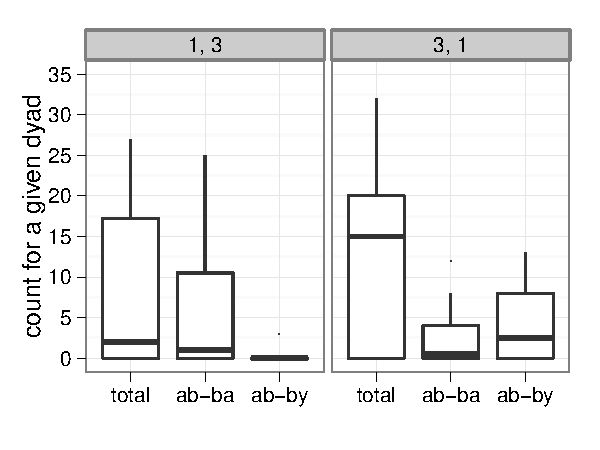
\includegraphics[scale=.5]{../figs/eckmann-small/example-obs-stats}
% %\caption{Observed counts}
% \end{subfigure}
% \qquad
% \begin{subfigure}[b]{0.35\textwidth}
% \centering
% 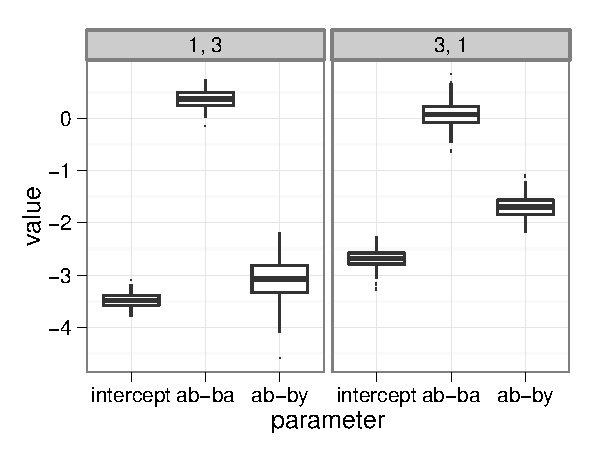
\includegraphics[scale=.5]{../figs/eckmann-small/example-estimates}
% %\caption{Samples of $\beta_{p,k,l}$}
% \end{subfigure}

% \caption{%Observed counts versus model estimates from Eckmann email data.
%  Left: Observed statistics across all dyadic email interactions between  members of group 1 and group 3.  Right: Posterior samples of the corresponding $\beta_{p,1,3}$ and $\beta_{p,3,1}$.  In addition to finding differences in mean activity for these dyads, estimates suggest events from 3 to 1 have a higher propensity for \texttt{ab-by} transitions.}
% \label{fig:posteriorparams}
% \end{figure}

\begin{figure}[t]
\centering
\begin{subfigure}[b]{0.22\textwidth}
\centering
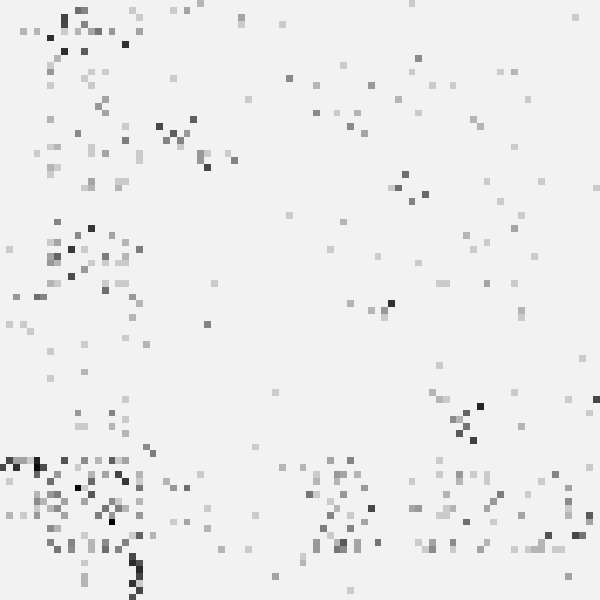
\includegraphics[scale=.25]{../figs/eckmann-small/parmat/observed}
\caption{Observed counts}
\end{subfigure}
~
\begin{subfigure}[b]{0.22\textwidth}
\centering
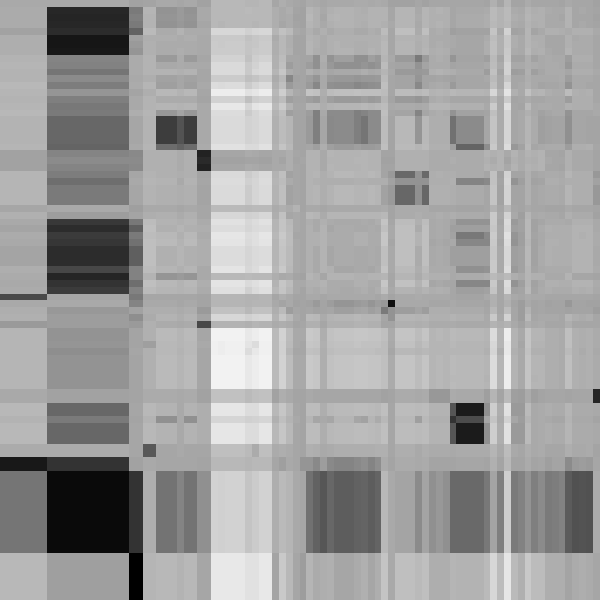
\includegraphics[scale=.25]{../figs/eckmann-small/parmat/1}
\caption{Intercept estimates}
\end{subfigure}
~
\begin{subfigure}[b]{0.22\textwidth}
\centering
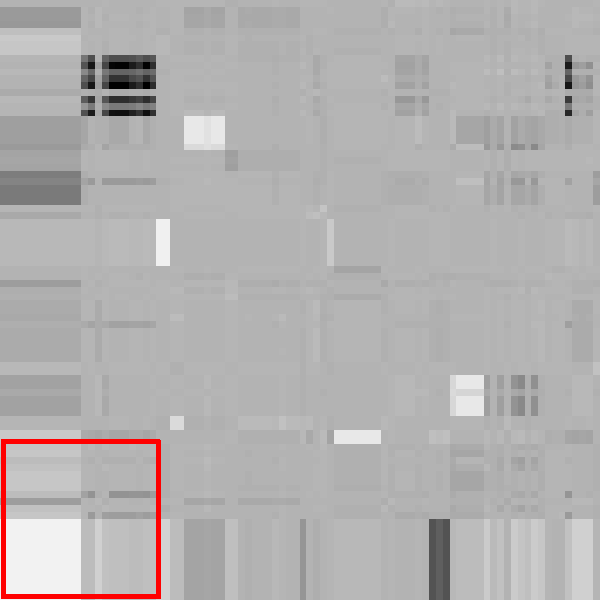
\includegraphics[scale=.25]{../figs/eckmann-small/parmat/2}
\caption{\texttt{ab-ba} estimates}
\end{subfigure}
~
\begin{subfigure}[b]{0.22\textwidth}
\centering
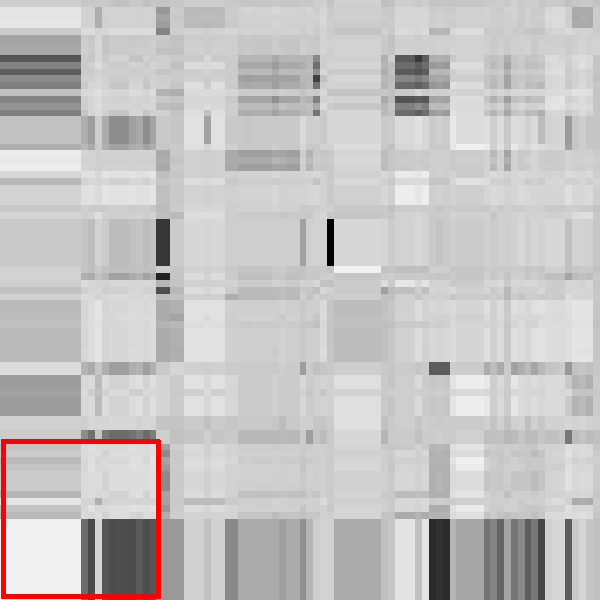
\includegraphics[scale=.25]{../figs/eckmann-small/parmat/3}
\caption{\texttt{ab-by} estimates}
\end{subfigure} \\
\begin{subfigure}[b]{0.22\textwidth}
\centering
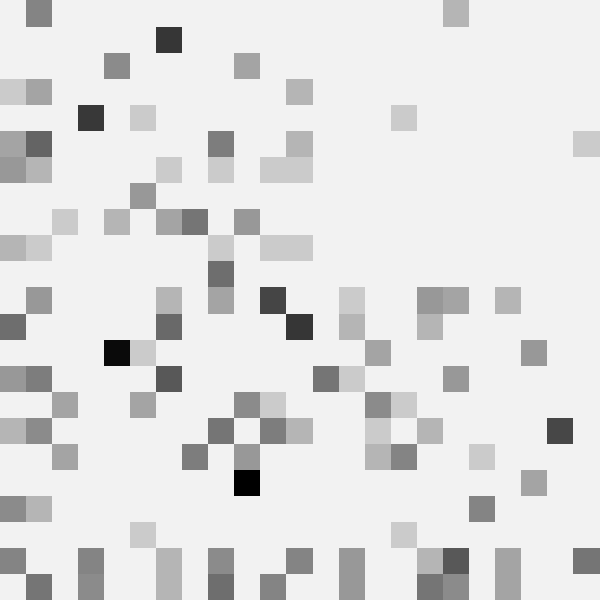
\includegraphics[scale=.25]{../figs/eckmann-small/parmat/observed-zoom}
\caption{Observed counts}
\end{subfigure}
~
\begin{subfigure}[b]{0.22\textwidth}
\end{subfigure}
\begin{subfigure}[b]{0.22\textwidth}
\centering
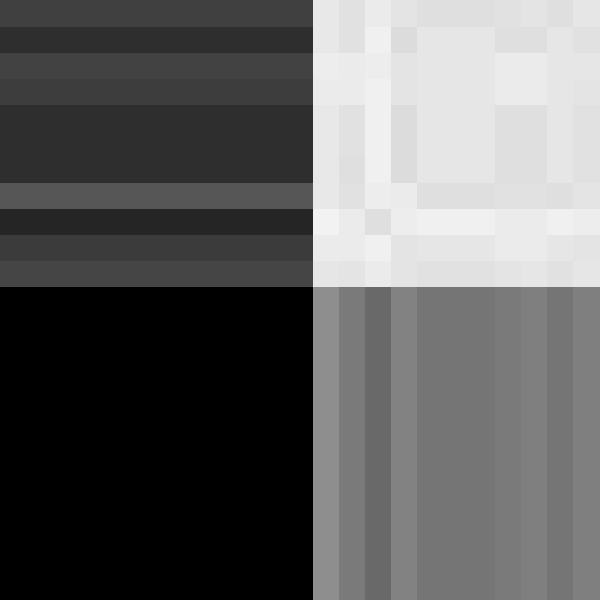
\includegraphics[scale=.25]{../figs/eckmann-small/parmat/1-zoom}
\caption{Intercept estimates}
\end{subfigure}
~
\begin{subfigure}[b]{0.22\textwidth}
\centering
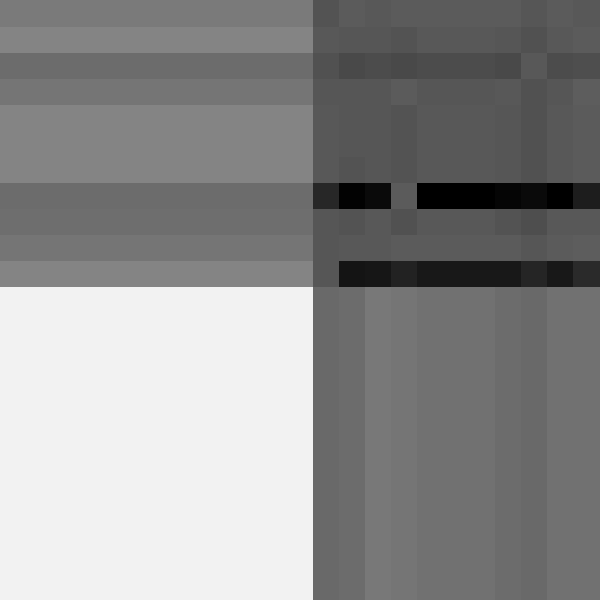
\includegraphics[scale=.25]{../figs/eckmann-small/parmat/2-zoom}
\caption{\texttt{ab-ba} estimates}
\end{subfigure}
\begin{subfigure}[b]{0.22\textwidth}
\centering
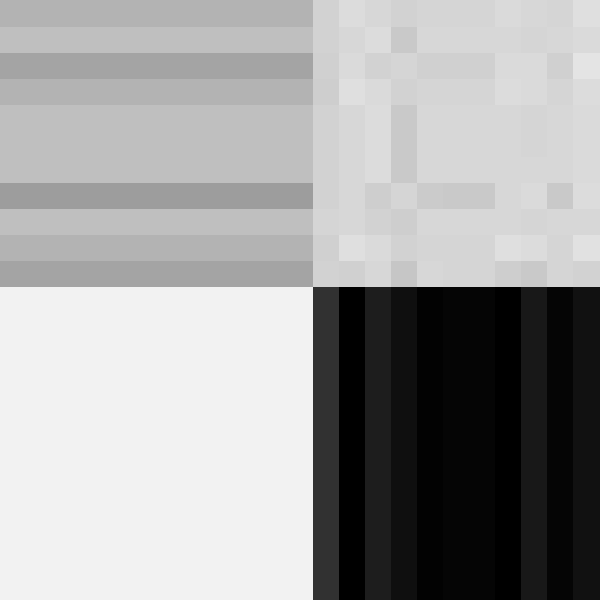
\includegraphics[scale=.25]{../figs/eckmann-small/parmat/3-zoom}
\caption{\texttt{ab-by} estimates}
\end{subfigure}
\caption{Comparing observed counts and parameter estimates.  Darker values are larger.  Estimates are rescaled posterior means $(\hat{\beta}_{z_i,z_j,p} - \hat{\mu}_p)/\hat{\sigma}_p$ for each dyad $(i,j)$.  Learned parameters suggest heterogeneity exists in both total activity (b) as well as dynamics, as seen in (c) and (d).  Figures (e-h) give a zoomed-in view of groups 1 and 3, showing that while the overall rate of (1,3) and (3,1) events is similar, the tendency for \texttt{ab-by} transitions differs.}
\label{fig:parmats}
\end{figure}

%PS: I would prefer to say: In this paper, we propose (or we proposed)�.
We propose a hierarchical approach for modeling event-based network data as a continuous-time Markov process. 
Our approach generalizes traditional static notions of stochastic equivalence on nodes (such as stochastic blockmodels) to a dynamic formulation. 
The proposed model posits the existence of groups of nodes, such that all members of a group are governed by the same dynamic process, and groups are differentiated by having different dynamic processes. 
%PS: sentence below is incomplete (after the first "the")�..I decided to take it out anyway..
% Given a specification for the, the proposed method employs latent variables to model the heterogeneity in the event dynamics.
%is analogous to recent hierarchical extensions for latent position models \cite{Handcock2007} and exponential random graph models \cite{Schweinberger2011}.
%The method combines a latent variable framework (stochastic blockmodels) with a local dependence model for event sequences (relational event models \cite{Butts2008}).
%This provides detailed models of event dynamics among subsets of nodes while allowing for heterogeneity in the dynamics of the network as a whole.

%This analysis suggests 
Our approach has the ability to uncover systematic differences in dynamic behaviors or roles among subsets of nodes.
% across a variety of data sets.
In Section \ref{sec:experiments} we show the model has improved predictive accuracy over baseline methods on real data with respect to ranking tasks and the likelihood of unobserved data.
In particular, we show that our proposed approach leads to improved predictive accuracy when compared to both (a) relational event models that lack latent clusters, and (b) stochastic blockmodels for count data, both of which are both special cases of our model.
Though prediction is not the main focus of the model, the results provide some evidence that having latent structure (i.e. K>1) can lead to improvements in predictive power. Our prediction results show that it is easy to overfit with this model. If we restrict to K=2 on these small data sets, we systematically outperform the K=1 model. % (TODO: confirm this).  
However, as K increases beyond 2 (e.g., for the unrestrained CRP prior), the model is prone to overfit. This is not surprising, given that the number of fitted parameters scales as the square of the number of components K in the model. A natural future direction worth exploring for this model is a class of priors that are more resistant to overfitting.  

Other theories could be explored by including relevant statistics in the specification of $\mathbf{s}(t,i,j,\mathcal{A}_t)$, and similarly one can use our method to study how the roles of these statistics vary across nodes.  
One interesting extension, analogous to \cite{Airoldi2008}, would allow the latent class $z_i$ to be drawn from node-specific membership vectors $\pi_i$  after each change point.  
We leave this to future work.
%Alternatively, if nodes change groups.
%In some contexts such extensions might be substantively important and warrant future work.


%Our method learns about event dynamics within latent groups of individuals, but other types of heterogeneity likely exist in some data sets.  
%For example, dynamics might change over time \cite{Vu2011}.


%^ (e.g., somehow have the priors  be sensitive to K^2 rather than K, as you mentioned yesterday).


%PS: not sure where this fits�seems out of place here�and needs to be rewritten to be clearer - its not clear why we are comparing to this model other than the fact that it appeared at NIPS last year and also talks about relational event data. One way to make its inclusion here more natural would to set this up by first stating that there are other modeling approaches for relational events (such as the Guna� work), and comment on whether our "block approach" could be applied there too (not sure this makes sense since the models are so different�). 

%PS: these last two paragraphs need to be finished�.
% Trivially extended to co-clustering applications and for directed data.
% Also useful for our model when nodes belong to one latent class as a sender but another latent class as a recipient.

